\chapter{}
A wavelet literally means a small wave. The term says a lot about wavelets nature. Wavelets are a family of functions which oscillates like wave and should be compactly supported. Additionally, the wavelet has zero mean, an amplitude begins at 0, increases and decreases to 0 again.

\begin{defn}
Wavelets are created by scaling and shifting of the, so called, mother wavelet $\psi(t)$. The child wavelets are defined as

\begin{equation}
\label{eq:wavelets}
\psi^{(a,b)}(t)=|a|^{-\frac{1}{2}} \psi\left(\frac{t-b}{a}\right). 
\end{equation}

\end{defn}


There are plenty of different mother wavelets, for example

\begin{figure}[h]
	\centering
	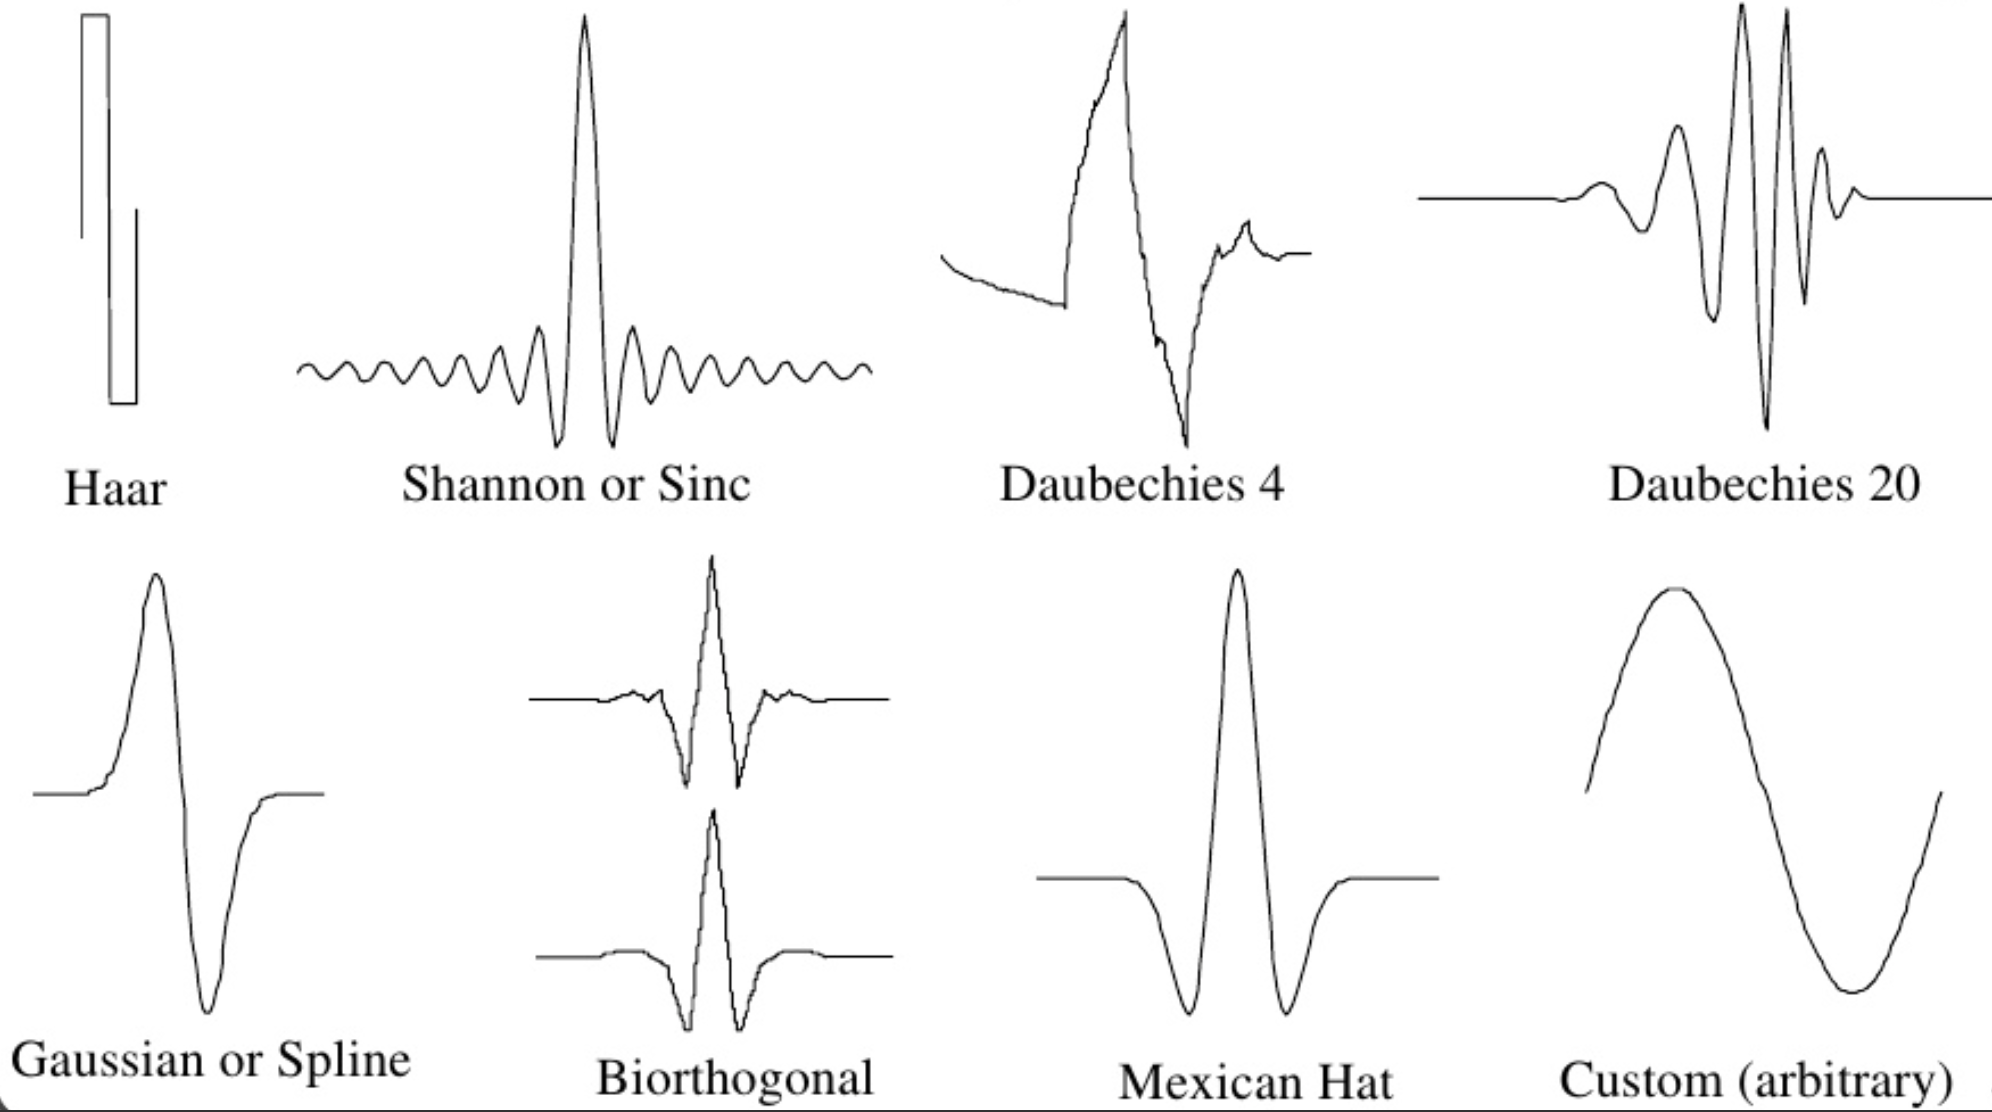
\includegraphics[width=\textwidth]{wavelets_with_bottom_line.png}
	\caption{Different types of wavelets.}
	\label{fig:wavelets}
\end{figure}

\textit{** Add more about wavelets properties **}

\section{Wavelet Transform}

\textit{** Add some short introduction **}

\begin{defn}
Wavelet transform

\begin{equation}
W(a,b)=\int_{-\infty}^{\infty} y(t) a^{-\frac{1}{2}} \psi\left(\frac{t-b}{a}\right) dt,
\end{equation}

where $a$ is scale parameter, $b$ translation parameter and $y(t)$ original signal.
\end{defn}

\subsection{Wavelet transform vs Fourier transform}

\begin{defn}
Fourier transform

\begin{equation}
Y(f)=\int_{-\infty}^{\infty} y(t) e^{-i\omega t} dt,
\end{equation}

where $y(t)$ is time domain signal and $Y(f)$ is frequency domain signal.
\end{defn}

\begin{table}[]
\centering
\begin{tabular}{|p{0.5\linewidth}|p{0.5\linewidth}|}
\toprule
\textbf{ Wavelet transform} & \textbf{Fourier transform}
\\ \midrule
Suitable for stationary and non-stationary signals 
& Suitable for stationary signals 
\\ \midrule
High time and frequency resolution
& Zero time resolution and very high frequency resolution     
\\ \midrule
Very suitable for studying the local behaviours of the signal
& No suitable  
\\ \midrule
Sine and cosine waves
& Scaled and translated mother wavelets
\\ \bottomrule
\end{tabular}
\end{table}

Wavelet transform is similar to the Fourier transform but with the different functions. In Fourier case there are sine and cosine functions, wherein wavelet transform uses wavelets.

Why use Wavelet transform?
Sine function oscillates on the whole real axis, thus it cannot represent abrupt changes. On the other hand, the Wavelet transform is localized in space and time, so it can be used to detect sudden changes in signals and images. Moreover, wide range of wavelet functions is a main advantage of wavelet analysis.

\section{Discrete Wavelet transform}
There are two types of the wavelet transform:
\begin{itemize}
\item Continuous Wavelet Transform (CWT),
\item Discrete Wavelet Transform (DWT).
\end{itemize}

DWT is used to denoising and compression of signals and images. Also, DWT allows to detect smooth regions interrupted by edges or abrupt changes in contrast of images.

Scale and translation parameters are defined as

\begin{equation}
a = 2^j \text{ and } b = 2^j k,\ j,k=1,2,\ldots.
\end{equation}

to avoid redundancy in coefficients.


The figure \ref{fig:DWT} on a page \pageref{fig:DWT} shows how DWT works. Discrete Wavelet Transform splits signal with two filters: $h(n)$ - high pass filter (HPF) and $g(n)$ - low pass filter (LPF). The HPF captures a part with bigger frequencies which is the main signal. Whereas, the LPF captures smaller frequencies - a noise of the signal. Subsequently, both parts are down sampled by a factor of 2. This decomposition can be repeated on the HPF part of the signal. Hence, the next levels of DWT coefficients.

\begin{figure}[h]
	\centering
	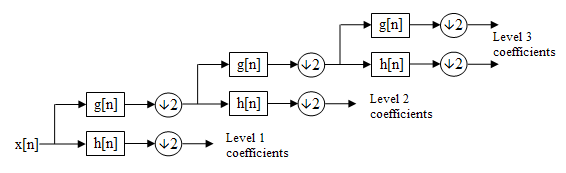
\includegraphics[width=\textwidth]{DWT.png}
	\caption{Discrete Wavelet transform on a signal $x(n)$.}
	\label{fig:DWT}
\end{figure}


\section{2-D Discrete Wavelet transform}

\textit{** Add introduction that 2D transform is for images and how it works **}

2-D Descrete Wavelet Transform works the same way as 1-D except that one level of the decomposition contains filtering columns and rows.

\begin{figure}[h]
	\centering
	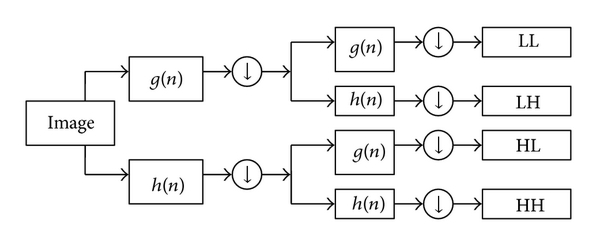
\includegraphics[width=\textwidth]{2D_DWT.JPG}
	\caption{2-D Discrete Wavelet transform on an image.}
	\label{fig:2D_DWT}
\end{figure}







